\documentclass[assignment = 4]{homework}

\usepackage{caption, subcaption, pdfpages, float}
\usepackage{graphics, wrapfig, pgf, graphicx}
\usepackage{enumitem}
\graphicspath{{../resultados/}}


% pacotes para importar código
\usepackage{caption, booktabs}
\usepackage[section, newfloat]{minted}
\definecolor{sepia}{RGB}{252,246,226}
\setminted{
    bgcolor = sepia,
    style   = pastie,
    frame   = leftline,
    autogobble,
    samepage,
    python3,
}
\setmintedinline{
    bgcolor={}
}

% ambientes de códigos de Python
\newmintedfile[pyinclude]{python3}{}
\newmintinline[pyline]{python3}{}
\newcommand{\pyref}[2]{\href{#1}{\texttt{#2}}}

% \SetupFloatingEnvironment{listing}{name=Código}
% \captionsetup[listing]{position=below,skip=-1pt}

\usepackage{csquotes}
\usepackage[style=verbose-ibid,autocite=footnote,notetype=foot+end,backend=biber]{biblatex}
\addbibresource{referencias.bib}
\usepackage[section]{placeins}

\usepackage[hidelinks]{hyperref}
\usepackage[noabbrev, nameinlink, brazilian]{cleveref}
\hypersetup{
    pdftitle  = {MC920 - Trabalho 4 - 187679},
    pdfauthor = {Tiago de Paula}
}

\newcommand{\textref}[2]{
    \hyperref[#2]{#1 \ref*{#2}}
}

\usepackage{import, multirow}
\usepackage{tikz}
\usetikzlibrary{matrix}
\usetikzlibrary{positioning}

\newenvironment{kmatrix}[1][1.3cm]{
    \begin{tikzpicture}[node distance=0cm]
        \tikzset{square matrix/.style={
                matrix of nodes,
                column sep=-\pgflinewidth, row sep=-\pgflinewidth,
                nodes={draw,
                    minimum height=#1,
                    anchor=center,
                    text width=#1,
                    align=center,
                    inner sep=0pt
                },
            },
            square matrix/.default=#1
        }
}{
    \end{tikzpicture}%
}

\newcommand*{\Scale}[2][4]{\scalebox{#1}{\ensuremath{#2}}}%

\newcommand{\red}[1]{\textcolor{red}{\textbf{#1}}}

% \date{1 de dezembro de 2020}

\begin{document}

    \pagestyle{main}

    % \input{textos/intro}

    % \input{textos/prog}

    % \input{textos/impl}

    % \section{Resultados}

%% TODO %%
%
% Geral
% x Assinatura [mon]
% x Texto Pequeno [mon][wat]
% - Texto Grande [bab|pep]
% - Binario (Imagem / Zip) [bab|pep]
%
% Permutado
% - Texto Pequeno [mon] -- Tamanho + Chave
% - Texto Grande [bab|pep]
% - ?: Binário
%
% Plano de bit
% - 0, 1, 2
% - ?: 3, 5, 7

\subsection{Técnica Padrão}

\subsubsection{Assinatura}

    Podemos ver pela \cref{fig:assinatura} que assinatura digitais, normalmente com menos de caracteres, são imperceptíveis na imagem como um todo. No plano de bit específico, a diferença também não é visível ao olho humano.

    O resultado na \cref{fig:assinatura:imagem} contém o texto ``Realizzato da Leonardo da Vinci™'', representado em UTF-8 por 35 bytes. Juntamente com o cabeçalho de 8 bytes, a assinatura ocupa 344 bits do plano menos significativo. Isso não chega a metade da primeira linha ($256 \times 3$ bits de capacidade).

    A imagem pode ser produzida por:

    \begin{minted}{bash}
        $ echo Realizzato da Leonardo da Vinci™ | python3 codificar.py imagens/monalisa.png -o saida.png
    \end{minted}

    E verficada com:

    \begin{minted}{bash}
        $ python3 decodificar.py saida.png
        Realizzato da Leonardo da Vinci™
        $ # OU
        $ python3 decodificar.py saida.png | diff -qs - <(echo Realizzato da Leonardo da Vinci™)
        Files - and /proc/self/fd/12 are identical
    \end{minted}

    \begin{figure}[H]
    \centering
    \begin{subfigure}{0.5\textwidth}
        \centering
        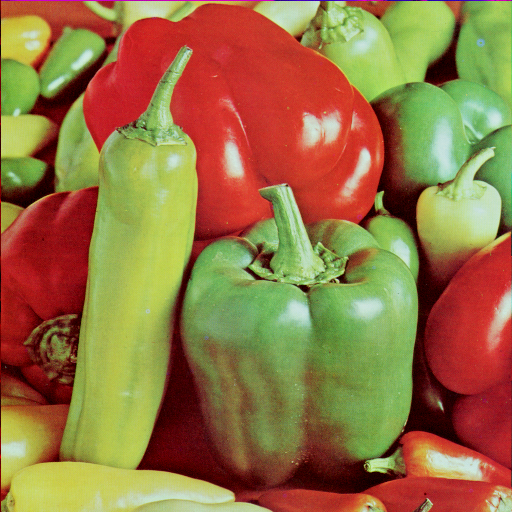
\includegraphics[width=0.85\textwidth]{mona_assin/imagem.png}
        \caption{Imagem com mensagem oculta.}
        \label{fig:assinatura:imagem}
    \end{subfigure}%
    \begin{subfigure}{0.5\textwidth}
        \centering
        \includegraphics[width=0.85\textwidth]{mona_assin/plano0.png}
        \caption{Plano 0.}
        \label{fig:assinatura:plano}
    \end{subfigure}\\[8pt]
    \begin{subfigure}{0.33\textwidth}
        \centering
        \includegraphics[width=0.85\textwidth]{mona_assin/pl0chb.png}
        \caption{Plano 0, canal azul.}
        \label{fig:assinatura:blue}
    \end{subfigure}%
    \begin{subfigure}{0.33\textwidth}
        \centering
        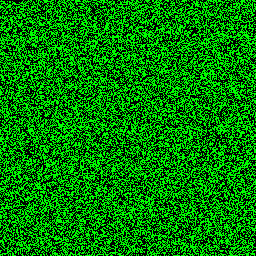
\includegraphics[width=0.85\textwidth]{mona_assin/pl0chg.png}
        \caption{Plano 0, canal verde.}
        \label{fig:assinatura:green}
    \end{subfigure}%
    \begin{subfigure}{0.33\textwidth}
        \centering
        \includegraphics[width=0.85\textwidth]{mona_assin/pl0chr.png}
        \caption{Plano 0, canal vermelho.}
        \label{fig:assinatura:red}
    \end{subfigure}%

    \caption{\texttt{monalisa.png} com uma assinatura de 35 bytes.}
    \label{fig:assinatura}
\end{figure}


    % \section{Conclusão}

\end{document}
